\section{Installation, Example Usage and Tutorial} \label{examples}
In this section, we illustrate the main functionality of \means{} by in a short tutorial.
Please, note that the tutorial instructions below are auto-generated from the interactive tutorial in the IPython notebook format. 
While the information is identical between both media forms, it may be more convenient to read the tutorial in the interactive form. \sauliustodo{Describe how to access interactive form of tutorial}

\subsection{Installation}

\sauliustodo[inline]{Installation instructions go here}


{   % These brackets are very important, btw.

    % IPython notebook likes to define their own colours...
    % And who could blame them.
    
    \definecolor{orange}{cmyk}{0,0.4,0.8,0.2}
    \definecolor{darkorange}{rgb}{.71,0.21,0.01}
    \definecolor{darkgreen}{rgb}{.12,.54,.11}
    \definecolor{myteal}{rgb}{.26, .44, .56}
    \definecolor{gray}{gray}{0.45}
    \definecolor{lightgray}{gray}{.95}
    \definecolor{mediumgray}{gray}{.8}
    \definecolor{inputbackground}{rgb}{.95, .95, .85}
    \definecolor{outputbackground}{rgb}{.95, .95, .95}
    \definecolor{traceback}{rgb}{1, .95, .95}
    % ansi colors
    \definecolor{red}{rgb}{.6,0,0}
    \definecolor{green}{rgb}{0,.65,0}
    \definecolor{brown}{rgb}{0.6,0.6,0}
    \definecolor{blue}{rgb}{0,.145,.698}
    \definecolor{purple}{rgb}{.698,.145,.698}
    \definecolor{cyan}{rgb}{0,.698,.698}
    \definecolor{lightgray}{gray}{0.5}
    
    % bright ansi colors
    \definecolor{darkgray}{gray}{0.25}
    \definecolor{lightred}{rgb}{1.0,0.39,0.28}
    \definecolor{lightgreen}{rgb}{0.48,0.99,0.0}
    \definecolor{lightblue}{rgb}{0.53,0.81,0.92}
    \definecolor{lightpurple}{rgb}{0.87,0.63,0.87}
    \definecolor{lightcyan}{rgb}{0.5,1.0,0.83}
    
    % Tutorials go here
    \input{autogenerated-tutorials}
}   % make sure to put them above this line


%\subsection{Model Definition}
%A common example of a kinetic system of the \pft{} tumour suppressor system.
%Whist relatively uncomplicated, it shows an interesting oscillatory behaviour and has been extensively studied \cite{geva-zatorsky_oscillations_2006, batchelor_ups_2009}.
%A simple version of this model can be formulated as a list of species; $p53$, $Mdm2$ and $Mdm2_p$ (precursor of $Mdm2$) and a list of reaction between species (fig.~\ref{fig:p53}).
%
%In addition, the number of molecules of each species used in each reaction (\emph{.i.e.} the net change) can be represented as a \emph{stoichiometry matrix}, $S$:
%
%\[
%\mathbf{S} =
%\begin{bmatrix}
%+1 & -1 & -1 & 0 & 0 & 0\\
%0 & 0 & 0 & +1 & -1 & 0\\
%0 & 0 & 0 & 0 & +1 & -1 \\
%\end{bmatrix}
%\]
%
%Finally, a vector of \emph{propensities}, $\mathbf{a}$, can be trivially derived (see \cite{gillespie_general_1976}, eqs. 14) from the stoichiometry and the reactions:
%\[
%\mathbf{a} =
%\begin{bmatrix}
%c_0\\
%c_1 y_0\\
%\frac{c_2 y_2 y_0}{y_0+c_6}\\
%c_3 y_0\\
%c_4 y_1\\
%c_5 y_2\\
%\end{bmatrix}
%\]
%where,\\
%$c_i$, are constant reaction rates,\\
%and $y_0$, $y_1$ and $y_2$ are $p53$, $Mdm2$ and $Mdm2_p$, respectively.\\
%   
%
%\begin{figure}
% \begin{subfigure}{0.3\textwidth}
%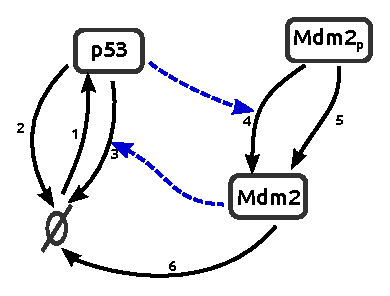
\includegraphics{handmade_figures/p53.eps}
%\caption{}
% \end{subfigure}
% \begin{subtable}{0.7\textwidth}
%\begin{scriptsize}
%  \begin{align*}
%p53~production && \emptyset\rightarrow p53 \\
%Mdm2~independent~p53~degradation && p53 \rightarrow \emptyset \\
%Mdm2~dependent~p53~degradation && Mdm2 + p53 \rightarrow Mdm2 \\
%p53~dependent~Mdm2~production && p53 + Mdm2_{p} \rightarrow p53 + Mdm2\\
%Mdm2~synthesis~from~precursor && Mdm2_{p} \rightarrow Mdm2 \\
%Mdm2~degradation && Mdm2 \rightarrow \emptyset \\
%\end{align*}
%\end{scriptsize}
%\caption{}
% \end{subtable}
%\caption{\emph{\pft{} model}.
%Graphical representation of the model (a). Each number indicates a different reaction.
%Blue arrows indicate mediation of a reaction by a species.
%(b) Detail of the six reactions.
%}
%\label{fig:p53}
%\end{figure}
%
%\subsection{Making a Model}
%\label{sec:making-a-model}
%
%Once the model has been mathematically characterised, it is straightforward to define it in \means:
%
%
%\begin{framed}
%\begin{minted}{python}
%import sympy
%import numpy as np
%import means
%
%# Defines the species as symbols
%species = sympy.symbols(['y_0', 'y_1', 'y_2'])
%# The soichiometry matrix as a numpy array
%stoichiometry_matrix = np.array([[1, -1, -1, 0, 0, 0],
%                                  [0, 0, 0, 1, -1, 0],
%                                  [0, 0, 0, 0, 1, -1]])
%
%# The constants/parameters
%parameters = sympy.symbols(['c_0', 'c_1', 'c_2', 'c_3', 'c_4', 'c_5', 'c_6'])
%
%# And the propensities as a list of expressions
%propensities = ['c_0',
%              'c_1*y_0',
%              'c_2*y_2*y_0/(y_0+c_6)',
%              'c_3*y_0',
%              'c_4*y_1',
%              'c_5*y_2']
%
%#Now we create a Model:
%MY_MODEL = means.Model(species, parameters,
%                       propensities, stoichiometry_matrix)
%print MY_MODEL
%\end{minted}
%\end{framed}
%
%\subsection{Generating an \gls{ode} Problem}
%\label{sec:approximation-example}
%After definition of the model as a \py{} object, it becomes possible to use MEA to generate a set of \gls{ode}s (\emph{i.e.} a problem):
%
%
%\begin{framed}
%\begin{minted}{python}
%problems_scalar = means.mea_approximation(MY_MODEL, max_order=2)
%# This is equivalent to
%# >>> problem_scalar = means.mea_approximation(MY_MODEL, max_order=2,
%#                                              closure="scalar", value=0)
%\end{minted}
%\end{framed}
%%~
%Here, we keep ODEs modelling moment up to second order. The options \texttt{closure="scalar"} and \texttt{value=0} mean we have assumed higher(than two)-order are equal zero.
%This is the assumption made in the original publication\cite{ale_general_2013}. In \means, it is also possible to derive higher-order moments from parametric distributions.
%
%\begin{framed}
%\begin{minted}{python}
%# Here we use log-normal parametric distribution, and upt to third order moment.
%# We could also use Normal and Gamma distributions
%problem_logn = means.mea_approximation(MY_MODEL, max_order=3,
%                                          closure="log-normal",
%                                          multivariate=True)
%                                          
%\end{minted}
%\end{framed}
%
%\subsection{Simulating Trajectories}
%\label{sec:example-simulation}
%By providing initial conditions $y_i(t=0)$, and values for the constants, it is possible to simulate the temporal dynamic of the system:
%
%
%
%\begin{framed}
%\begin{minted}{python}
%#Simulation with a common solver (cvODE)
%simulator = means.Simulation(problem_scalar, solver='cvode')
%
%#Values for c_0, c_1, ..., c_6
%constants = [90, 0.002, 1.7, 1.1, 0.93, 0.96, 0.01]
%initial_conditions = [70, 30, 60]
%#we want to simulate up to t=100
%time = np.arange(0, 100, 0.01)
%
%#Generate trajectories for this parameters and initial conditions
%trajectories = simulator.simulate_system(constants, initial_conditions, time)
%\end{minted}
%\end{framed}
%
%
%Our package integrates with \plt{} to represent trajectories in a straightforward manner(fig.~\ref{fig:trajectories_exple}):
%
%\begin{framed}
%\begin{minted}{python}
%import matplotlib as plt
%plt.figure()
%trajectories.plot()
%plt.show()
%#We can also plot the inference result
%inference_result.plot()
%\end{minted}
%\end{framed}
%
%\begin{figure}
%\includegraphics[width=1.0\textwidth]{../pipeline/task-output/FigurePlotTrajectExple/FigurePlotTrajectExple-pdf.pdf}
%
%\caption{\emph{Representing Trajectories}.
%Exemple representation of the trajectories for the \pft{} system.
%First order moments (top-panel) are the average number of molecules, second order moments (bottom-panel) are variances and covariances.
%}
%\label{fig:trajectories_exple}
%\end{figure}
%
%
%Finally, an important feature of \means{} is parameter inference.
%The overall goal of inference is to vary parameters in order to find "the" set of parameters for which the distance to observed trajectories is minimal.
%In this senario, observed trajectories could have been experimentally recorded at regulat time intervals:
%
%\begin{framed}
%\begin{minted}{python}
%#Construct observed trajectory
%observed_values = np.array([ 
%        301. ,  290.2,  280.6,  272. ,  264.4,  257.6,  251.4,  245.9,
%        241. ,  236.6,  232.6,  229. ,  225.7,  222.8,  220.1,  217.7,
%        215.5,  213.5,  211.8,  210.1,  208.7,  207.3,  206.1,  205. ,
%        204. ,  203.1,  202.3,  201.6,  200.9,  200.3,  199.7,  199.2,
%        198.7,  198.3,  197.9,  197.6,  197.3,  197. ,  196.7,  196.5])
%
%\end{minted}
%\end{framed}
%
%In the simplest case, starting parameters and initial values are chosen.
%Then, some parameters can be explicitely allowed to vary:
%
%\begin{framed}
%\begin{minted}{python}
%#Starting parameter values
%start_parameters = [90, 0.002, 1.7, 1.1, 0.93, 0.96, 0.01]
%#Starting concentrations of each species
%initial_conditions = [70, 30, 60]
%#Parameters and accordant range that the user wants to vary
%variable_parameters = {'c_2':(0,10),'c_4':(0,10)}
%        
%timepoints = timepoints = np.arange(0, 40, 0.1)
%description = problem_scalar.descriptor_for_symbol('y_0')
%observed_trajectory = means.Trajectory(timepoints,
%                                       observed_values,
%                                       description)
%inference = means.Inference(problem_scalar, start_parameters, 
%                            initial_conditions, variable_parameters, 
%                            [observed_trajectory])
%
%#Obtain inference result
%inference_result = inference.infer()
%\end{minted}
%\end{framed}
%
%\subsection{Use in an interactive environment}
%\todo{Screenshots from Ipython notebook go here}
%

